\section{Syntax of \lang{}}
\label{sec:syntax}

\begin{bnf}
    \ntsym{program} ::=  (& \ntsym{import} | \ntsym{typedef} | \ntsym{function} \\
    |& \ntsym{automaton} | \ntsym{system})^*
\end{bnf}

In the following subsections, we are going to take a simple \emph{queue} as an example, to illustrate how certain language elements are used to compose a model.

\subsection{Type System}
\label{subsec:typesystem}
\lang{} provides a rich-featured type system that supports various commonly-used data types in both formal modeling languages and programming languages.

\vspace{0.3em}
\noindent\emph{Primitive Type.} Table. \ref{table:primitivetypes} shows the primitive types supported in \lang{}.

\begin{table}
    \caption{Primitive Data Types}
    \label{table:primitivetypes}
    \centering
    \begin{tabular}{lcr}
        \hline
        Name & Declaration & Term Example \T\B \\
        \hline
        \T Bounded Integer\hspace{0.5cm} & \texttt{int lowerBound .. upperBound}\hspace{0.5cm} & \texttt{-1,0,1} \\
        Integer & \texttt{int} & \texttt{-1,0,1} \\
        Real & \texttt{real} & \texttt{0.1, 1E-3} \\
        Boolean & \texttt{bool} & \texttt{true, false} \\
        Character & \texttt{char} & \texttt{'a', 'b'} \\
        \B Enumeration & \texttt{enum {item$_1$, ..., item$_n$}} & \texttt{enumname.item} \\
        \hline
    \end{tabular}
\end{table}

\noindent\emph{Composite Type.} Composite type offers an approach to contruct complex data types with simpler ones. Several composite patterns are introduced as follows,

\begin{table}
    \caption{Composite Data Types (\texttt{T} denotes an arbitrary data type)}
    \centering
    \begin{tabular}{lr}
        \hline
        Name & Declaration \T\B \\
        \hline
        \T Tuple  & \texttt{T$_1$,...,T$_n$ }\\
        Union & \texttt{T$_1$|...|T$_n$ } \\
        Array & \texttt{T [length]}\\
        Slice & \texttt{T []} \\
        Map & \texttt{map [T$_{key}$] T$_{value}$} \\
        Struct\hspace{1cm} & \texttt{struct \{ field$_1$:T$_1$,..., field$_n$:T$_n$ \}} \\
        \B Initialized & \texttt{T$_{base}$ init term} \\
        \hline
    \end{tabular}
\end{table}

\begin{itemize}
    \item \emph{Tuple}. The \emph{tuple} operator `,' can be used to construct a finite tuple type with several base types.
    \item \emph{Union}. The \emph{union} operator `$|$' is designed to combine \emph{disjoint} types as a more complicated one. This is similar to the union type in C language but much easier to use.
    \item \emph{Array} and \emph{Slice}. An \emph{array} $T[n]$ is a finite ordered collection containing exactly $n$ elements of type $T$. Moreover, a \emph{slice} is an array of which the capacity is not specified, i.e. slice is a dynamic array.
    \item \emph{Map}. A \emph{map }[$T_{key}$] $T_{val}$ is a dictionary that maps a key of type $T_{key}$ to a value of type $T_{val}$.
    \item \emph{Struct}. A \emph{struct }\{$field_1:T_1,\cdots,field_n:T_n$\} contain $n$ fields, each has a particular type $T_i$ and a unique identifier $id_i$.
    \item \emph{Initialized}. A initialized type make it able to specify default values to types.
\end{itemize}

For simplicity in formalizing data types, we introduce the concept \emph{domain} of a type. 

\begin{formalization}[Domain]
    We use $Dom(T)$ to denote the value domain of type $T$, i.e. the set of all possible value of $T$.
\end{formalization}

\begin{example}[Types Used in A Queue] Now let us introduce some type declarations and local variables used in an automaton \texttt{Queue}. As shown in the following code fragment, we declares a singleton enumeration \texttt{NULL}, which contains only one element \texttt{null}. The buffer of a queue is in turn formalized as an array of \texttt{T} or \texttt{NULL}, indicating that a queue element can be either an assigned item or empty. The head and tail pointer are defined as two bounded integers.
\begin{lstlisting}
typedef enum {null} init null as NULL;
automaton <T:type,size:int> Queue(A:in T, B:out T) {
    variables {
        buf : ((T | NULL) init null) [size];
        phead : int 0 .. (size - 1) init 0;
        ptail : int 0 .. (size - 1) init 0;
    }
    ...
}
\end{lstlisting}
\end{example}

\subsection{Functions}

The abstract syntax tree of functions is shown as follows.
\begin{bnf}
    \ntsym{funcDecl} ::= & \tsym{function} \ntsym{template}^? \ntsym{identifier} \tsym{(} \ntsym{arguments} \tsym{)} \tsym{\{} \\
    & (\tsym{variables} \tsym{\{} \ntsym{varDecl}^* \tsym{\}})^? \\
    & \tsym{statements} \tsym{\{} \ntsym{assignStmt}^* \ntsym{returnStmt} \tsym{\}} \\
    \ntsym{assignStmt} ::= & \ntsym{term} \tsym{:=} \ntsym{term} \\
    \ntsym{returnStmt} ::= & \tsym{return} \ntsym{term} \\
    \ntsym{varDecl} ::= & \ntsym{identifier} \tsym{:} \ntsym{type} (\tsym{init} \ntsym{term})^? 
\end{bnf}
Basically, definition of a function includes:
\begin{itemize}
    \item An optional template including a set of parameters. A parameter can be either a type parameter (decorated by \texttt{type}) or a value parameter (decorated by its type). All possible parameter values of a function should be located statically.
    % TODO: how?
    Parameters in the template can be used in all the following language elements, e.g. type of input variables and return value, local variables and function statements.
    \item An identifier that indicates the name of this function.
    \item A set of read-only input variables.
    \item A optional set of local variables.
    \item A list of ordered statements that describes how the return value is calculated. Such a list must be ended by a \texttt{return} statement.
\end{itemize}
Functions in \lang{} are side-effect free. In other words, only local variables are writable in its assignment statements.
\begin{example}[Incline Operation on a Queue Pointer] The simple function describes how pointers are inclined. When a pointer is going to exceed its upper bound (determined by the parameter \emph{size}), we will reset it to zero.
    \label{exp:successor_function}
    \begin{lstlisting}
function <size:int> next(pcurr:int 0..(size-1)) : int 0..(size-1) {
    statements { return (pcurr + 1) % size; }
}
    \end{lstlisting}
\end{example}

% TODO: a more complicated function

\subsection{Automata : The Basic Behavioral Unit}

\begin{bnf}
    \ntsym{automaton} ::=& \tsym{automaton}\ntsym{template}^?\ntsym{identifier} \tsym{(} \ntsym{port}^* \tsym{)} \tsym{\{}\\
    & (\tsym{variables} \tsym{\{} \ntsym{varDecl}^* \tsym{\}})^? \\
    & \tsym{transitions} \tsym{\{} \ntsym{transition}^* \tsym{\}} \tsym{\}} \\
    \ntsym{port} ::=& \ntsym{identifier} \tsym{:} (\tsym{in}|\tsym{out}) \ntsym{type} \\
    \ntsym{transition} ::=& \ntsym{guardedStmt} | \tsym{group} \tsym{\{} \ntsym{guardedStmt}^* \tsym{\}}\\
    \ntsym{guardedStmt} ::=& \ntsym{term} \tsym{->} (\ntsym{stmt} | \tsym{\{} \ntsym{stmt}^* \tsym{\}}) \\
    \ntsym{stmt} ::=& \ntsym{term} \tsym{:=} \ntsym{term} | \tsym{perform} \ntsym{identifier}^+
\end{bnf}

\vspace{0.2cm}
\noindent \emph{Template.} Very similar to functions, a automaton can also be decorated with a set of template parameters, either value parameters or type parameters.

\vspace{0.2cm}
\noindent \emph{Ports.} Each automaton contains a set of ports, either \texttt{in}-coming or \texttt{out}-going, to communicate with the environment. To ensure the well-defineness of automata, ports are required to have an \emph{initialized} type, e.g. \texttt{int 0..1 init 0} instead of \sout{\texttt{int 0..1}}.

\vspace{0.2cm}
\noindent \emph{Variables.} Two types of variables are used in a automaton definition, they are:
\begin{enumerate}
    \item \emph{Local variables} that are declared in the \emph{variables} section. A local variable can only be referenced in its scope, i.e. the automaton definition. And similar to the ports, only initialized types are permitted when declaring local variables.
    \item \emph{Adjoint variables} that are used to describe the status of ports. For a port A, we assume that it has two boolean fields \texttt{A.reqRead} and \texttt{A.reqWrite} indicating if there is a pending \emph{read} or \emph{write} request on this port, and a data field \texttt{A.value} indicating the current value of this port (if a write operation is performed, \texttt{A.value} will be reassigned).
\end{enumerate}

A reasonable rule comes up that, both the \texttt{reqWrite} field of a input port and the \texttt{reqRead} field of a output port are \emph{read-only}. Similarly, we cannot rewrite the \texttt{value} field of a input port.

\smalltitle{Transitions} Similar to the PRISM\cite{KwiatkowskaCav2011} language, behavior of a channel in \lang{} is described by a series of guarded transitions (groups). As shown in  Example \ref{exp:trans_queue}, a \emph{transition} comprises two parts: a boolean term \emph{guard} that shows on what condition the transition could be fired, and a (set of) statement(s) that describe what will happen if the transition is fired. Two types of statements are supported in automata,
\begin{itemize}
    \item \emph{Assignment Statements} (\texttt{var$_1$,...,var$_n$ := term$_1$,...,term$_n$}). Local variables and writable adjoint variables are permitted to be assigned here. We can also assign several variables at the same time (similar to the tuple assignment in Python).
    \item \emph{Perform Statements} (\texttt{perform port$_1$,...,port$_n$}). Informally speaking, perform statements tell the environment to fire data operations on the output ports, or wait until being noticed that data operation on the input ports are fired by the environment (other automata, actually). Consequently, it's reasonable to require that the value of an input port should never be referred until the port is performed. Similarly, the value of an output port should never be assigned after the port is performed. Perform statements are mainly used when combining multiple automata, where they determine how transitions are synchronized. (See in Section \ref{subsec:composition})
\end{itemize}

When guard of a transition is satisfied by the context, we say the transition is \emph{activated}. However, being activated is only necessary condition of being fired. When choosing a transition to fire, we have to consider other criteria, which will be introduced later.

Though not mentioned explicitly, transitions can be divided into two classes: \emph{external} and \emph{internal}. A transition is \emph{external} iff. perform assignments are involved. 

\begin{formalization}[Transitions]
Formally, we use $g\rightarrow S$ to denote a transition, where $g$ is the guard formula and $S=\{s_1,\cdots,s_n\}$ is a set of statements. 
\end{formalization}

Here we present an example to show how transitions are used to model the behavior of a queue.
\begin{example}[Transitions in Queue] In a \texttt{Queue}, we use internal transitions to formalize the changes of its state. For example, becoming writable when buffer is not full, and readable when buffer is not empty. External transitions, on the other hand, mainly show how the read and write operations are performed.
\begin{lstlisting}
// Internal Transitions
true -> B.reqWrite := (buf[ptail] != null) ;
true -> A.reqRead  := (buf[phead] == null) ;

// External Transitions
(A.reqRead && A.reqWrite) -> {
    perform A; buf[phead] := A.value; phead := next(phead);
}
(B.reqRead && B.reqWrite) -> {
    B.value := buf[ptail]; ptail := next(ptail); perform B;
}
\end{lstlisting}
\label{exp:trans_queue}
\end{example}

All the transitions are supposed to have the following features. They are declared on the syntax level, i.e. we will resolve this feature when discussing the formal aspect of \lang{} and use a simple and standard automata model to capture all these features (see in Section. \ref{sec:semantics}).

\begin{itemize}
    \item \emph{Alterative}. A transition won't be fired if it changes nothing in its context. For example, the first internal transition in a \texttt{Queue} will not be activated if \texttt{B.reqWrite} is already equal to \texttt{buf[ptail] != null}. This assumption is mainly used to avoid useless executions.
    \item \emph{Urgent}. In some formal models, e.g. CSP\cite{HoareCsp1985} and Timed Automata\cite{AlurTcs1994}, transitions may not be triggered even the guard is satisfied. On contrast, such behavior is strictly prohibited in our model. Once a transition is activated (i.e. its guard is satisfied), it have to be fired unless another guard with higher priority is also activated.
    \item \emph{Ordered}. An automaton may includes a set of transitions. They are ordered by their appearance. In other words, if several transitions are activated at the same time, the literally former one will be fired first.
\end{itemize}

Priority of transitions make the automaton fully deterministic. However, in some cases non-determinism is still rather necessary. \emph{Transition groups} are, consequently, imported to represent such behavior. Transitions in the same group do not follow the ordering rule. Instead, the group itself is literally ordered w.r.t. other groups and ungrouped transitions.

\begin{formalization}[Transition Groups]
    A transition group $t_G$ can be formalized as a finite list of guarded transitions
    \[
        t_G=\{t_1,\cdots, t_n\}, t_i=g_i\rightarrow S_i
    \]
    where $t_i$ is a single transition with guard $g_i$ and a set of statements $S_i$.
\end{formalization}

Since a single transition $g\rightarrow S$ can be equivalently written as a singleton group $\{g\rightarrow S\}$, it's acceptable if we assume that each automaton comprises a set of transition groups but no standalone transitions.

\begin{formalization}[Automata]
    We use a tuple $A=\langle Ports, Vars, Trans_G \rangle$ to represent an automaton, where $Ports$ is a set of ports, $Vars$ is a set of local variables and $Trans_G=\{t_{G_1},\cdots,t_{G_n}\}$ is a set of transition groups.
\end{formalization}

\subsection{System : The Composition Approach}
\label{subsec:system}

Theoretically, an automaton in \lang{} is powerful to represent any classical software system (without consideration of time and probability, of course). However, modeling complex systems in transitions and tons of local variables may become a real disaster. That's why we are going to introduce a new block, called \emph{system}, to help reuse existing automata (systems as well), and construct clear and comprehensible high-level models.

% TODO: add references
To solve this problem, hierarchical diagrams are widely used in various modeling tools (SCADE\cite{AbdullaISoLA2006,BerryScp1992}, Simulink and LabVIEW) and formal languages (Reo\cite{ArbabMscs2004}, AADL). In such diagrams, blocks can be declared as \emph{components} and organized by a set of connections to capture more powerful behavior, where these connections are called \emph{channels}. Figure. \ref{fig:diagram} gives a simple diagram of a message-oriented middleware, where a queue work as a connector to coordinate between the components (message producers and consumers).
% TODO maybe not so commonly known?

\begin{figure}
    \centering
    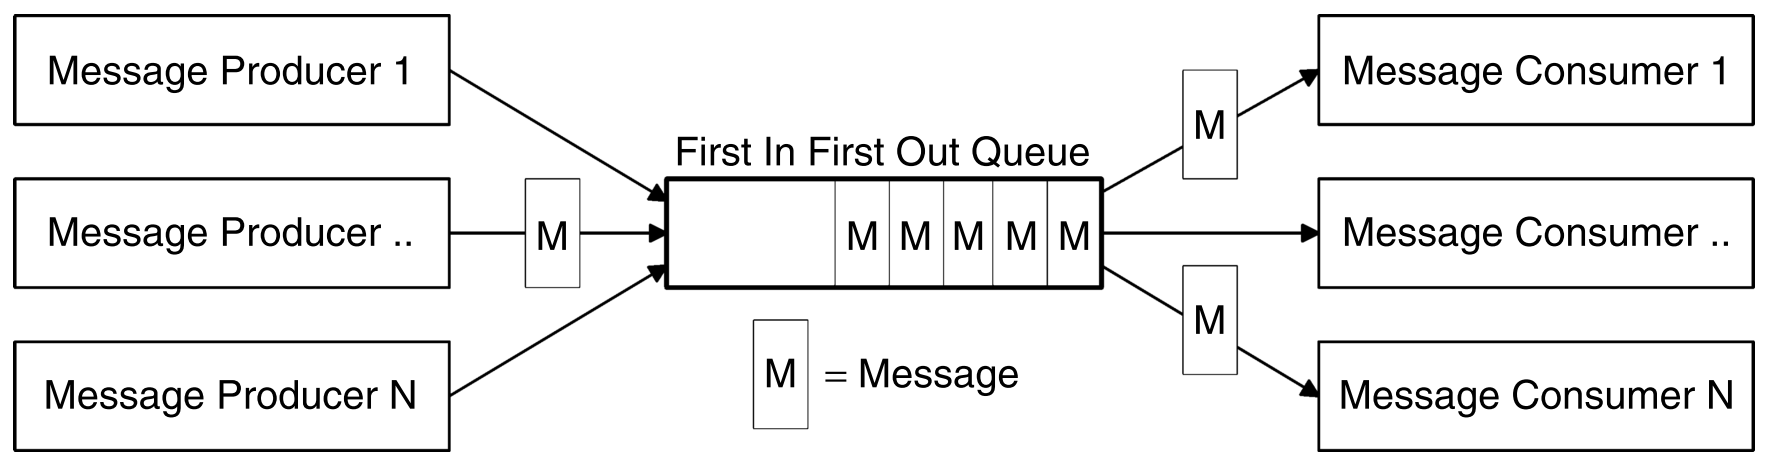
\includegraphics[width=.8\textwidth]{images/middleware_queue.png}
    \caption{A Senerio where Queue is used in Message-Oriented Middleware\cite{CurryMfc2004}}
    \label{fig:diagram}
\end{figure}

Both \emph{components} and \emph{connectors} (or \emph{channels}) are well-known concepts in component-based software engineering. Though having different names, their semantics all turn out to the same nature, \emph{automata}. Following with the idea, we introduce a compositional block named \emph{system}, where automata can be declared as either components or connections. The abstract syntax tree of systems is shown as follows.
\begin{bnf}
    \ntsym{system} ::= & \tsym{system} \ntsym{template}^?\ntsym{identifier} \tsym{(} \ntsym{port}^* \tsym{)} \tsym{\{}\\
    & (\tsym{internals} \ntsym{identifier}^+)^? \\
    & (\tsym{components} \tsym{\{} \ntsym{componentDecl}^* \tsym{\}})^? \\
    & \tsym{connections} \tsym{\{} \ntsym{connectionDecl}^* \tsym{\}} \tsym{\}}\\
    \ntsym{componentDecl} ::= & \ntsym{identifier}^+ \tsym{:} \ntsym{systemType} \\
    \ntsym{connectionDecl} ::= & \ntsym{systemType} \ntsym{params} \tsym{(} \ntsym{portName}^+ \tsym{)}
\end{bnf}

The interface of a system (i.e. its template, name, and ports) shares exactly the same form and meaning with interfaces of automata, which also implies that system is NOT a special semantics unit, but simply an compositional approach to pile up automata. A system is composed of internal nodes (optional), components(optional) and a set of connections.

\smalltitle{Components} Automata can be declared as components in a system. Ports of a component can be referred simply by \texttt{component.portname} where \emph{portname} is the identifier used in its declaration. 

\smalltitle{Connections} Connections, e.g. the arrows in Figure. \ref{fig:diagram}, are used to connect the ports of components.
Both components and connections are supposed to execute concurrently as automata.

\smalltitle{Internals} Directly connecting one port to another is far from enough when modeling complicated systems. For example, in Figure. \ref{fig:diagram} queue work as a connection between consumers and producers. However, since connections to the middleware are dynamically established or disconnected, we still need an extra merger (from producers to the queue) and an extra replicator (from the queue to the consumers) to achieve our goal. When defining internal nodes, we don't have to specify their types. They should be automatically solved by \lang{}.

\begin{example}[\lang{} Model of the System in Figure. \ref{fig:diagram}] In the previous figure, a simple scenario is presented where a queue is used as a message-oriented middleware. To model this scenario, we need two automata \emph{Producer} and \emph{Consumer} (definitions are omitted due to space limit) that produce or consume message of type \emph{T}.
\begin{lstlisting}
automaton <T:type> Producer (OUT: out T) { ... }
automaton <T:type> Consumer (IN: in T) { ... }

system <T:type> middleware_in_use () {
    components {
        producer_1, producer_2, producer_3 : Producer<T>;
        consumer_1, consumer_2, consumer_3 : Consumer<T>;
    }
    internals { M1, M2 }
    connections {
        Merger<T>(producer_1.OUT, producer_2.OUT, producer_3.OUT, M1);
        Queue<T>(M1, M2);
        Replicator<T>(M2, consumer_1.IN, consumer_2.IN, consumer_3.IN);
    }
}
\end{lstlisting}
\end{example}

Since the example is rather trivial, all the connections and components are automata here. But since automata and systems share the same form of interface, it's also valid to use systems as connections or components.

\label{subsec:functions}